\section{Results and Discussion}
\label{sec:results}

\subsection{The lowest reliably observable masses for given stellar densities
and distances.}

\begin{figure*}

    \centering
    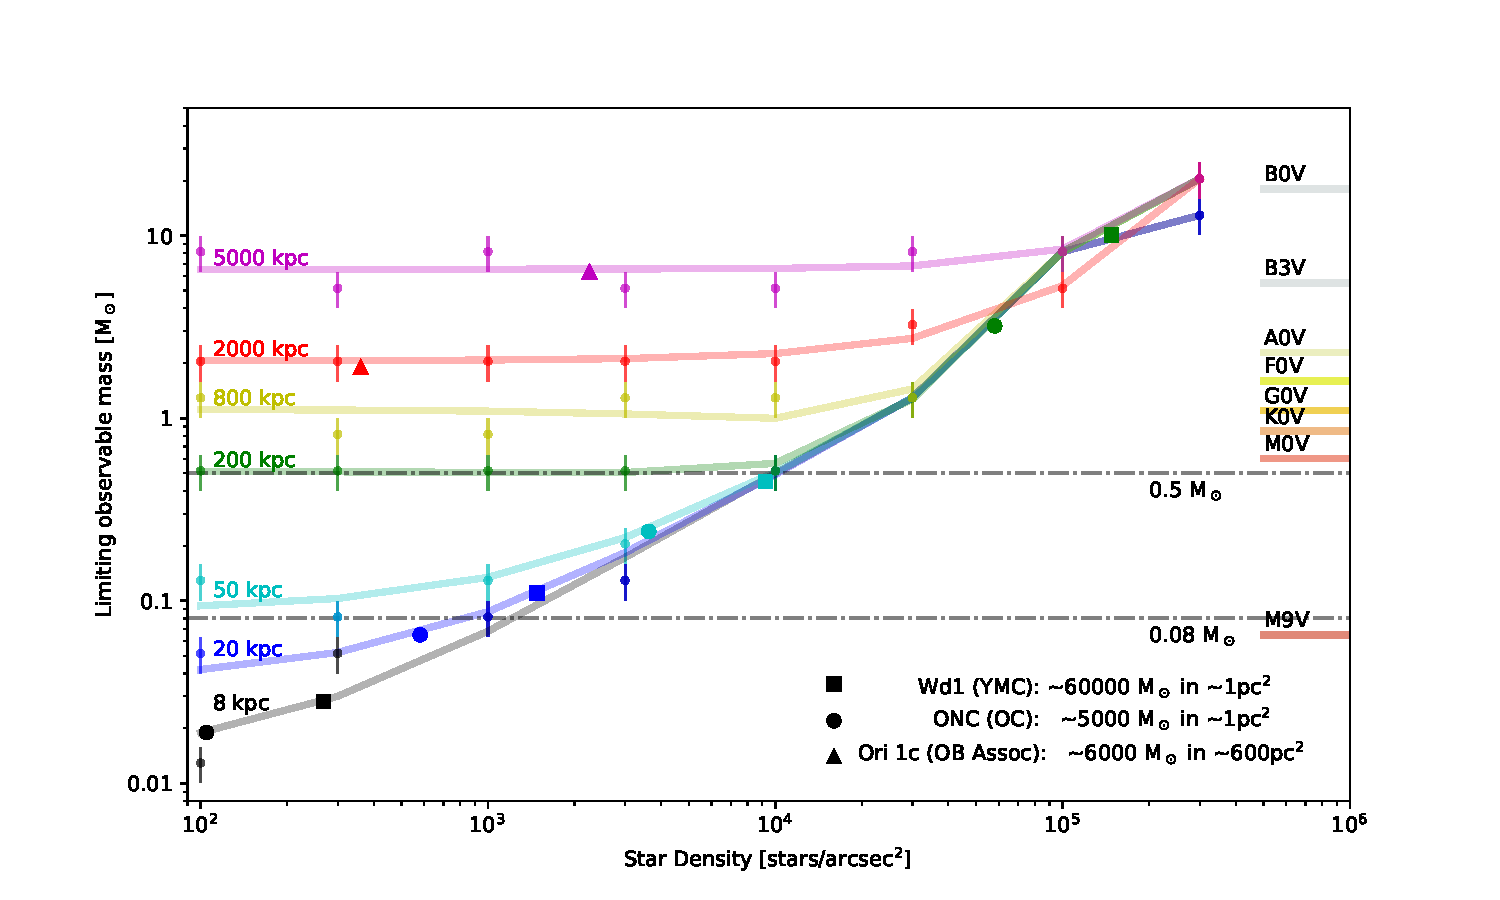
\includegraphics[width=\textwidth]{images/old_trusted_mass.pdf}

    \caption{This graph is the answer to the first question we posed: what is the lowest observable mass for given stellar densities and distances? 
    The errors in the observable mass are 0.2 dex and correspond to the size of the mass bins used. 
    Two trends are visible in the best fit lines for each distance: the flat regime shows that the limiting mass is based on the sensitivity limit of MICADO, while the exponential regime shows where crowding becomes the limiting factor. 
    The cavity to the lower right shows the parameter space in which stars of a given mass will not be observable.
    Here the stellar density includes all the stars in a given area down to 0.01\,\msun, not just the stars above the sensitivity limit. 
    Hence for the cases where observations are sensitivity limited, the effective observable star density is, in the cases with greater distance, much lower. 
    In these cases the stars below the sensitivity limit only contribute to a higher background flux.}
    
    \label{fig:trusted_mass}
    
\end{figure*}

\begin{figure*}

    \centering
    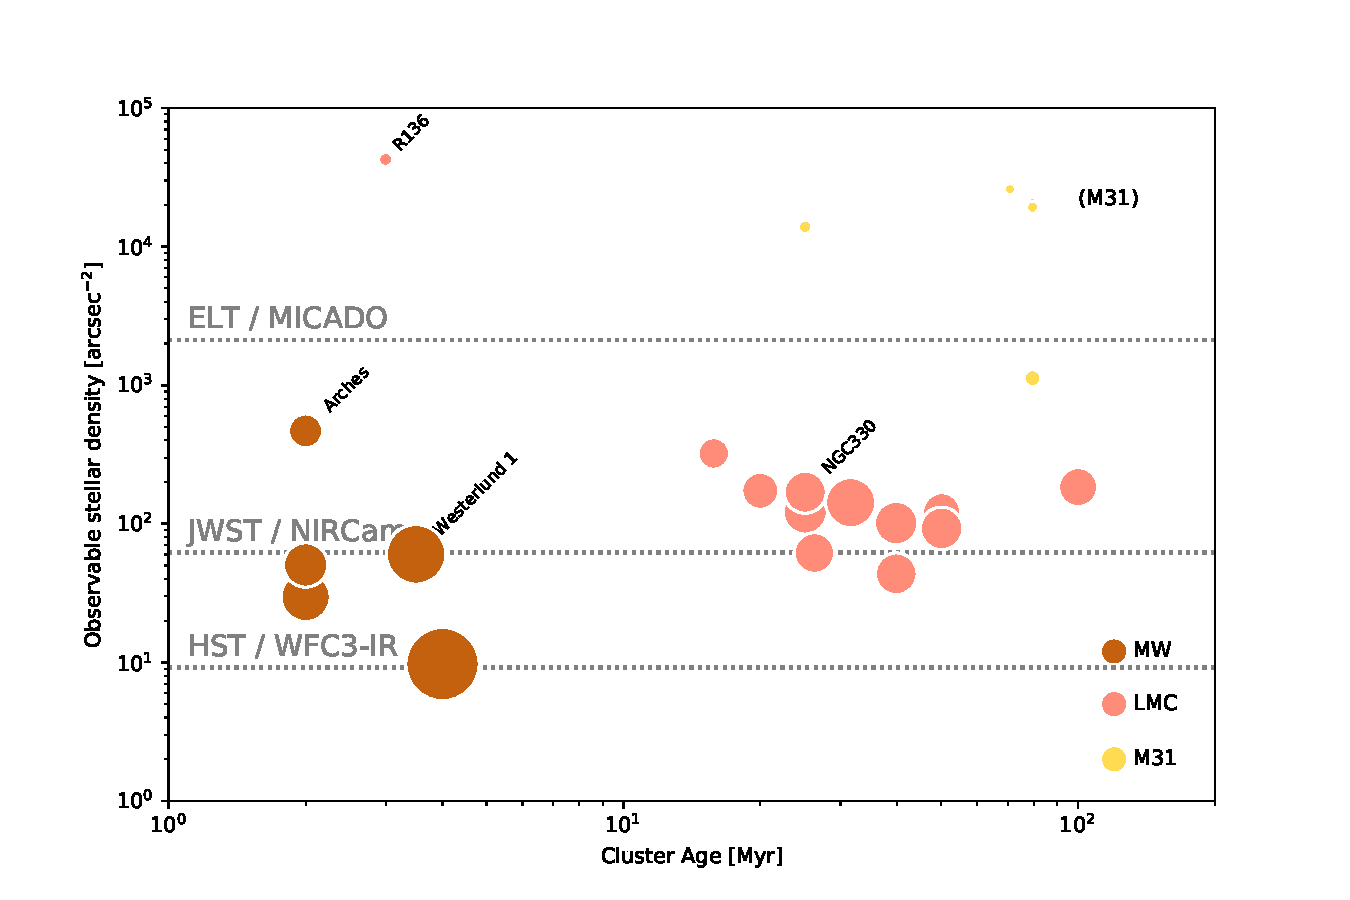
\includegraphics[width=\textwidth]{images/star_density_vs_age.pdf}

    % Add reference to that this is all-sky sample of YMCs
    % Note that all clusters apart from M31 will be accessible to MICADO

    \caption{
    The stellar densities in the cores of the young massive clusters listed in Table \ref{tbl:pz10_selection} assuming a sensitivity limit of K$_S$=28\m. 
    While these clusters are spread over the whole sky, it is noteworthy that only the handful of YMCs in M31 are outside the observing range of the ELT. 
    The size of the circles is proportional (including an offset) to the relative on-sky size of the cluster cores. 
    The colours reflect the lowest possible reliably observable mass, as shown in Figure \ref{fig:trusted_mass} and listed in Table \ref{tbl:pz10_selection}. 
    Brown: M\textgreater0.01\msun; Pink: M\textgreater0.1\msun; Yellow: M\textgreater0.9\msun. 
    The densities shown here take into account the sensitivity limit and therefore are only for the potentially observable stars, i.e. any low luminosity stars with K$_S$\textgreater28\m are omitted from the density calculation. 
    This is equivalent to all stars in the Milky Way, M-class stars and brighter in the LMC, and G-class stars and brighter in M31. 
    Only clusters from \citet{portegies2010} which have a defined core radius, r$_c$, are shown.
    The dashed lines in this figure represent the (estimated) limit to the resolving capability of the HST, JWST and ELT. 
    We define the limiting density as the mean distance between stars being equal to 2$\times$ the H-band PSF FWHM.
    Given the predicted PSF shapes for the latter two telescopes, these lines may prove to be somewhat optimistic. 
    Nevertheless the graphic illustrates the point that cores of the majority of young clusters outside the Milky Way are far too dense for either HST or JWST observations.
    Thus it will require the ELT (or similar) to study the most heavily populated regions of these clusters.}
    
    \label{fig:star_density_vs_age}
    
\end{figure*}


The first of the questions we asked with this study -- ``What is the lowest mass star that MICADO will be able to observe reliably for a given density and distance?'' -- can be answered by Figure~\ref{fig:trusted_mass}. 
For each of the distances and densities we have plotted the lowest reliable mass bin. 
The scatter in the plot reflects the random nature of the simulations. 
The positions of the stars in each of the stellar field were randomised, the sampling of the mass function was random and detector and shot noise was applied to the image as part of SimCADO's read-out process. 
Thus no two stellar fields were the same. 
Each stellar field configuration was only run once. 
We therefore only have one data point for each density and distance. 
The bin size used for the reliability statistics was set to 0.2 dex, and is the uncertainty in the limiting observable mass.

From Figure \ref{fig:trusted_mass} we can immediately see the two limiting regimes of sensitivity and crowding. 
The flat parts of the curves in Figure \ref{fig:trusted_mass} show the densities for which MICADO will be sensitivity limited at each distance and the diagonal regions show when crowding becomes the limiting factor. 
For example observations of a cluster at a distance of 8\, kpc observations will always be crowding limited for densities above 100\,\spae.
At a distance of 200\,kpc observations will be limited by sensitivity up to a density of 10\h4\,\spa, thereafter crowding will be the dominant factor. 
At 5\, Mpc all observations will be sensitivity limited. 
As a reference we have included the approximate stellar densities for three well known young  clusters in Figure~\ref{fig:trusted_mass} \textit{if they were located at the distance of the simulated clusters}. 
For example, if the YMC Westerlund 1 were to be located in the LMC, it would fall in to the crowding-limited regime for MICADO.
The lowest reliably observable mass in the densest region of the core would only be \s0.5\,\msun. 
This is equivalent to what HST is capable of observing in the outer rim territories of LMC clusters. For clusters in the LMC with stellar densities less than 10\h3~\spa MICADO will be limited by sensitivity to masses above 0.1\,\msun. 
While this mass is only 0.3\,\msun lower than what current Hubble observations can achieve, it should be emphasised that this increase of ``only'' 0.3\,\msun will reveal the majority of M-type stars, which account for almost three quarters of all main sequence stars \citep{ledrew2001}. 
Given that the limit of current studies is around the 0.5\,\msun knee from \citet{kroupa2001}, opening up this range will allow future studies to pin down exactly what the shape of the IMF looks like in the dense cores of young LMC clusters.

As previously noted the exposure time for the simulated images was one hour. 
By observing for longer times, the lowest observable mass will decrease, however the change is disproportionate to the exposure time. 
Additional ``observations'' with SimCADO showed that increasing the exposure time from 1 to 10 hours per cluster only increases the sensitivity limit by around 1.5\m and 1\m in the J and K$_S$ filters respectively. 
For the case of the LMC, this would decrease the lowest observable mass to around 0.06\msune, i.e. just below the hydrogen burning limit.

It should be noted that the majority of young clusters have cores less dense than that of Westerlund 1, and therefore the limiting observable mass will also be lower than the 0.5\,\msun mass quoted for a Westerlund 1-like YMC in the LMC. 
Given MICADO's resolving power it will be possible to determine to what extent apparent mass segregation has played a role in previous studies of the IMF in the LMC \citep{Ascenso2009-de}.
More to the point MICADO will enable us to understand the apparent deviations from the Salpeter IMF as reported by \citet{dario2009}, \citet{geha2013} and \citet{kalirai2013}.

% At these distances MICADO **would** be able to 
% Mention that ideal case is not possible, but that the older population can be resolved between 100-and 200 kpc down to 0.5 Msun

At distances of 100\,kpc to 200\,kpc and with careful photometry and longer observations MICADO should be able to detect stars down to the sensitivity limit of 0.5\,\msun. 
This will only be possible though for stellar densities less than 10\h4 \spa. 
As a reference an ONC-like cluster at a distance of 200\,kpc would have a stellar density on the order of 10\h5 \spa. 
Such observations would be useful for determining the composition of OB associations and sparser (older) open clusters, if there were any present in the non-Magellanic satellites of the Milky Way. 
Nevertheless MICADO will still allow us observe the power-law break at 0.5\,\msun in the field population of the nearest low metallicity dwarf spheroidal galaxies.

Closer to home MICADO should be able detect 10\,M$_{Jup}$ objects in a ONC-like clusters at a distance of 8\,kpc (along low extinction lines of sight). 
An obvious candidate for studies of the IMF in extreme environments is the Arches cluster, given its proximity to the galactic centre.
The main hindrance to deep observations of the Arches cluster is, somewhat counter-intuitively, not the \textgreater2 magnitudes of variable Ks-band extinction along the line of site \citep{espinoza2009}, but rather the \textgreater350 stars in the cluster \citep{galacticnucleaus} brighter than the saturation limit for MICADO\footnote{A MICADO internal analysis shows that point sources with magnitudes K$_S$\textgreater14.8\,\m will saturate the MICADO detectors within the 2.6\,s minimum exposure time.}.
Indeed there are very few regions in the cores of Milky Way open clusters which do not contain stars brighter than the saturation limit, making deep MICADO observations of these regions difficult.


\subsection{The core densities of young star clusters}

The second of the questions we asked with this study was ``What instrumental effects will play a critical role when undertaking such studies with MICADO and the ELT?''. 
The instrumental effect which plays the largest role by far regarding the accuracy of the estimates given here is our knowledge of the PSF.
For this study we used a single SCAO PSF. 
We assumed that the PSF orientation stayed the same for the length of the observation.
Consequently we had a very good model of our reference star for the PSF subtraction. 
This will obviously not be the case for real observations as the pupil of the telescope will rotate with respect to the sky, causing an axial broadening of the PSF over the course of an observing run. 
This broadening should improve the results from our subtraction method as it will smooth out many of the sharp features of the instantaneous PSF that lead to false positive detections. 
Information on both the structure of the PSF and the extent of the wings will however be lost due to the rotational broadening. 
Thus the PSF subtraction algorithm will less accurately be able to estimate the background level when fitting the reference PSF to a star. 
As a consequence faint stars caught in the PSF wings of the brighter stars may not be detected as often as they would be if the PSF remained rotationally aligned with the sky. 
To extract the most stars possible given the shape of the ELT PSF we propose the following hybrid approach: Subtract the brightest stars from each individual exposure using an instantaneous PSF derived from the brightest stars in that exposure, then stack the residual images and extract the faintest stars using a rotationally broadened PSF.
Further investigation is required to determine whether this approach would indeed increase the detection rate for faint stars.

Although it may seem obvious, it is worth mentioning that regardless of the PSF shape, it is clear from our simulations that resolving stellar densities of 10\h3\,\spa is well within the capabilities of MICADO. 
With an optimised PSF fitting and subtraction algorithm, extracting upwards of 5$\times$10\h3\,\spa should also be in the realms of possibility. 
This is equivalent to approximately one star in an area equivalent to \s2.5 ELT H-band PSF FWHMs. 
This is similar to being able to resolve every star in the core of an ONC-like cluster in the LMC. 
For JWST and HST the equivalent stellar densities are only 160~\spa and 20~\spa respectively. 
Although MICADO may not have the sensitivity of a space-based telescope, the resolving power will give us full access to the core populations of dense stellar clusters in the major satellites of the Milky Way.


\subsection{Opportunities and targets for future observations with MICADO and the ELT}


\begin{figure*}

    \centering
    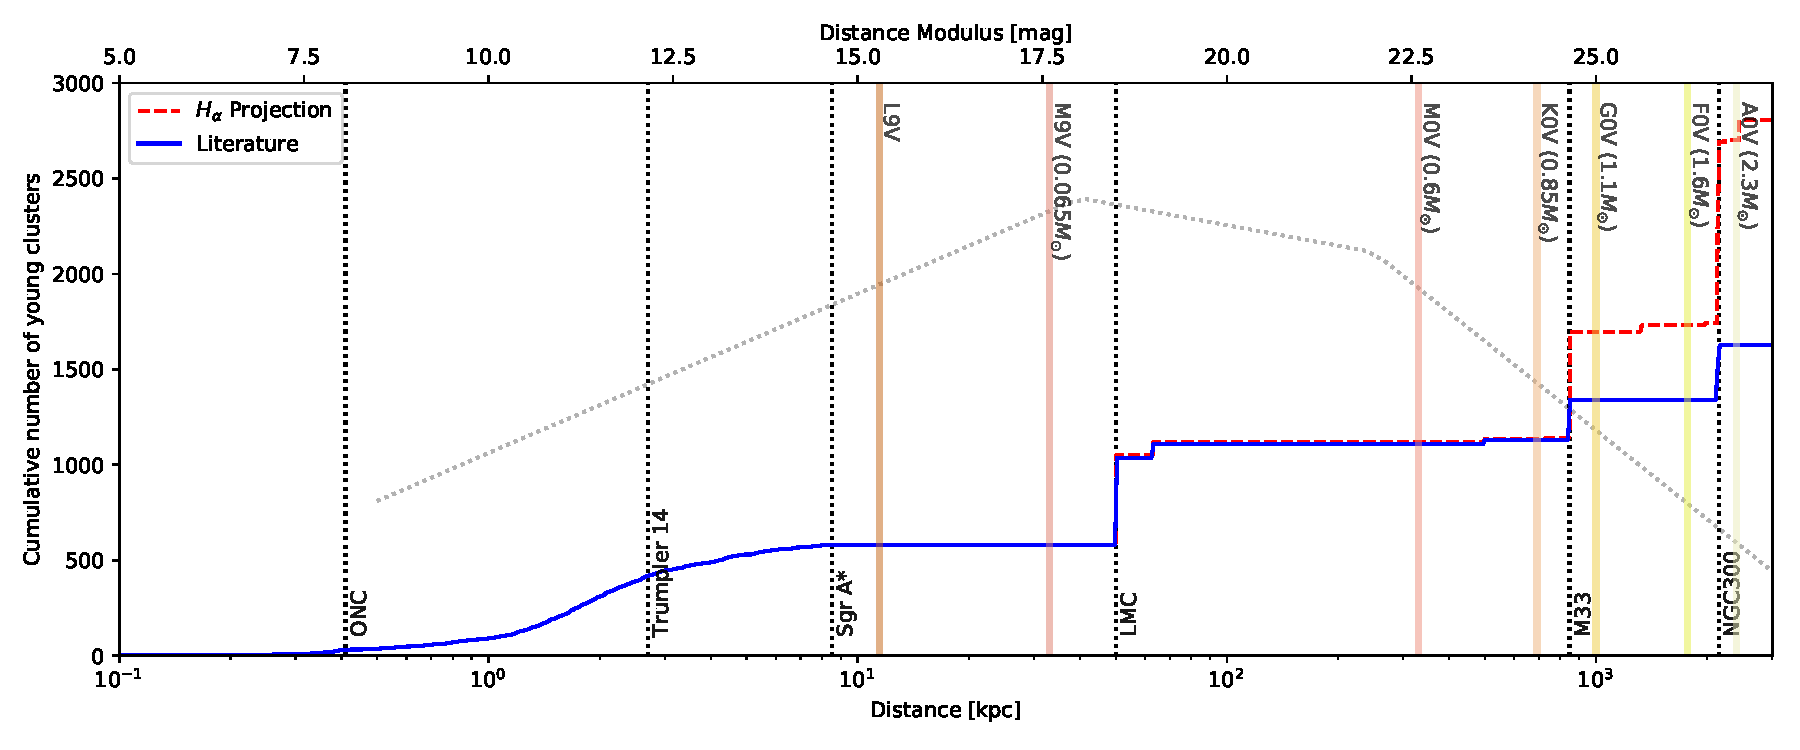
\includegraphics[width=\textwidth]{images/young_clusters_within_2Mpc_incl_MW.pdf}

    \caption{Cumulative number of young cluster targets that will be available to MICADO (\textdelta\,\textless\,+35\textdegree) out to 2 Mpc. The blue line show the cumulative number of young clusters with increasing distance from Earth as reported in catalogues and the literature (see references in Table \ref{tbl:cum_cluster_refs}.
    The red dotted line shows the expected number of young clusters in a given galaxy based on an extrapolation of a galaxy's star formation rate from its total H$_\alpha$ flux \citep{caldwell09}.
    The solid vertical lines represent the observational horizons for given stellar spectral types assuming a detection limit of K=28$^m$ with MICADO at the ELT. The faint dotted grey line shows the corresponding approximation distance limits for determining the slope of various regions of the IMF using MICADO.
    The population of Milky Way clusters is taken from the HEASARC Milky Way Open Cluster database \citep{heasarc_mwsc} and represents only the clusters located at declinations accessible to MICADO (-85\textdegree\,\textless\,\textdelta\,\textless\,+35\textdegree)
    }
    \label{fig:local_group_cluster_number}

\end{figure*}


These simulations are a nice theoretical exercise, however without an application to observations they are not all that useful.
Figure~\ref{fig:star_density_vs_age} shows the estimated stellar densities in the cores of the open clusters and YMCs compiled by \citet{portegies2010}. 
The density values, log$_{10}$($\rho$), only take into account the stars with apparent magnitudes above the sensitivity limit of MICADO and thus reflect the ``real'' observable density for the clusters (also listed in Table \ref{tbl:pz10_selection}). 
The limits set for HST, JWST and MICADO are the critical stellar density above which our extraction algorithm struggles to detect and remove more than 90\% of the stars in a field. 
We find that for the Galactic clusters, the resolution of JWST will be sufficient to resolve all stars in most cluster cores down to the sensitivity limit of the instrument.

For clusters in the galactic plane though JWST observations will struggle to disentangle the cluster stars from the field stars. 
To robustly determine cluster membership, observations of the proper motion of the cluster relative to the field will be required. 
\citet{stolte2008} show that the proper motion of the Arches cluster near the Galactic centre is \s5\,mas yr\h{-1}. 
This equates to around a sixth the size of a pixel in the JWST NIRCam instrument. 
MICADO, in contrast, will have a plate scale of 1.5\,mas in the high resolution mode, meaning that cluster membership could be determined by observations spaced only several months apart. Greater certainty regarding cluster membership will greatly increasing the accuracy of estimates of the cluster IMF based on star counts.

Further afield, resolving the cores of the massive young clusters in the Magellanic clouds will not be possible with JWST. MICADO however will enable access to these cluster cores, which in turn will open up to possibility to study the dynamical processes (e.g. evaporation, core collapse, etc.) involved in the evolution of extra-galactic clusters. 
Additionally observations of a series of LMC clusters with varying ages will give a much better picture of how the initial mass function evolves into the present day mass function, and how the dynamical evolution of the cluster influences the observations, and calculations of, a cluster's IMF.


\citet{portegies2010} provides a curated list of the most well known massive young clusters in- and outside the Milky Way. However many more clusters exist within the local group of galaxies. 
Indeed to fully understand the environmental dependence on cluster formation and evolution, a statistically large number of extra-galactic clusters will need to be observed. 
Figure \ref{fig:local_group_cluster_number} shows the pool of clusters available to MICADO at the ELT along with the corresponding observational limits of stars of various masses. 
Within the Mily Way alone, over 500 star clusters become available for which a fully resolved IMF (including the Brown Dwarf regime) could be determined. 
If the Magellanic clouds are included for studying the region either side of the IMF peak, this number increases to over 1000 young cluster targets. 
Out to 2Mpc the resolved high-mass slope of the IMF could be studied in between 1500 and 2500 clusters, including up to 1000 new previously undocumented star clusters\footnote{This estimate is based on each galaxy's total H$_\alpha$ flux with the conversion to approximate number of clusters based on the H$_\alpha$ derived star formation rate and young cluster catalogue for M31 \citep{caldwell09}.}.

MICADO will enable IMF studies of fully resolved populations to move from direct IMF measurements of single clusters in and around the solar neighbourhood to statistically large numbers of clusters in a diverse set of environments both in- and outside the Milky Way. Such a statistically meaningful sample of resolved IMFs will hopefully enable a robust determination of any environmental parameters that influence the star formation process, thus answering the major open question of IMF universality.

% The blue curve in Figure \ref{fig:local_group_cluster_number} shows the cumulative number of possible MICADO targets reported in catalogues and the literature for both the Milky Way and in galaxies out to 2 Mpc (for references see Table A\ref{tbl:cum_cluster_refs}). 
% The red dotted curve adds the approximate number of additional clusters in the local group which have not yet been catalogued. 
% 
% What is evident from Figure \ref{fig:local_group_cluster_number} is that there
% exist hundreds (potentially thousands) of clusters within a 2 Mpc radius that will
% be observable by MICADO, which could be used for a statistical analysis of the IMF
% under varying environmental conditions. 



% Milky way cluster numbers are taken from the HEASARC MWOCDB
% Extra-galactic cluster numbers are taken from the references in table 

% Makes a plot of cumulative star formation vs distance. This SFR is converted
% into an "average number of clusters", assuming the 140 M31 number of SF regions
% can be equivalent to a SFR of 0.5 Msun / yr.
% See Caldwell 2009 \citep{caldwell09}, 140 young clusters in M31 @ 0.5 Msun/yr

% The number of galaxies that will be seen by MICADO are limited by the latitude
% of Armazones: -25 deg +/- 60 deg --> [-85, +35]


% \begin{figure*}

%     \centering
%     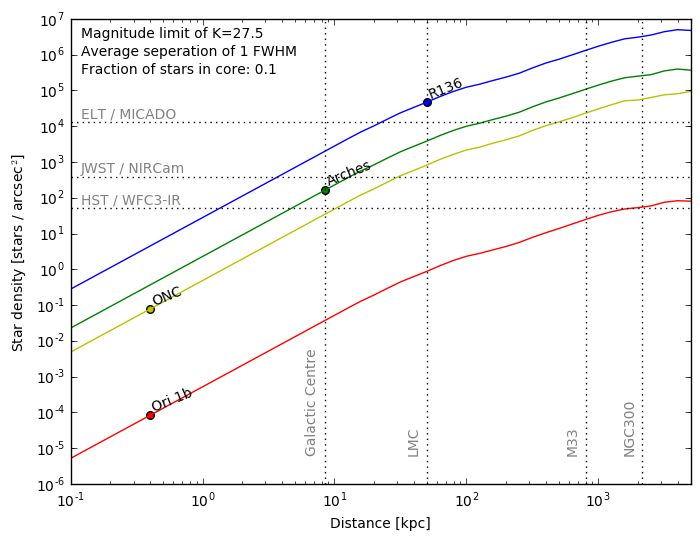
\includegraphics[width=\textwidth]{images/star_density_motivation}

%     \caption{}
    
%     \label{fig:resolved_stellar_densities}
    
% \end{figure*}


% What is the lowest mass star that MICADO will be able to observe for a given density and distance? 
% How crowded can a region be for MICADO to still be able to detect 90% of the stars above the detection limit? 
% What instrumental effects will play a critical role when undertaking such studies with MICADO and the ELT?


% Results}
% - 
% * ELT PSFs make life very difficult - many fake sources
% * MICADO can get well into the Brown dwarf regime (>0.01Msun) for all clusters within 8kpc of the Sun
% * It will just miss out on the BD knee in the LMC (>0.1Msun). But it will catch the true structure of the 0.5Msun knee.
% * Densities of ~1000 stars/arcsec2 are easily resolvable. 5000 stars/arcsec2 if we have good knowledge of the PSF.
% * This is equivalent to every star in the Arches cluster at a distance of the LMC. ONC would be fully resolvable (assuming no extinction) in Leo I Dwarf (220kpc)
% * in the LMC, meaning MICADO can basically resolve out all stars in every YMC listen in Portegeis-Zwart 2010



% NEED COMPLETENESS NUMBERS - HOW MANY ACTUALLY CAME BACK!!!!

    % - At what densities does the PSF subraction break down?

    % - At what desntites do we start getting fake sources from the PSF artifacts?

% - What is the limiting mass vs distance vs stellar density

% - What are the effective densities for the cases where the limiting mass is resolution limited?
% - Where does JWST drop out?

    % - Examples of the clusters (i.e. ONC in NGC300) where MICADO will make the biggest contribution
    
% - What level of variation in each mass regime (M<0.08, 0.08<M<0.5, M>0.5) do we see?
